\documentclass{article}
\usepackage{graphicx} % Required for inserting images
\usepackage{authblk} % For author affiliations
\usepackage{hyperref} % For hyperlinks
\usepackage[margin=1in]{geometry} % Standard margins
\usepackage{natbib} % For bibliography management
\usepackage{enumitem} % For customising lists
\usepackage{color}
\usepackage{amsmath}

\newlist{tree}{itemize}{10}
\setlist[tree]{label=-}
\setlistdepth{10} 


\title{Integrating Multiple Data Sources in Infectious Disease Modelling: Best Practices and Implementation}

\author[1]{Sam Abbott}
\author[2]{Xiahui Li}
\author[3]{Punya Alahakoon}
\author[4]{Dhorasso Junior Temfack Nguefack}
\author[5]{Johannes Bracher}
\author[6]{Felix Günther}
\author[7]{@working-group-members}
\author[8]{@workshop-participants}
\author[9]{Mircea T. Sofonea}
\author[10]{Michael Plank}
\author[11]{Anne Presanis\thanks{Joint last authors}}
\author[12]{Anne Cori$^*$}

\affil[1]{London School of Hygiene \& Tropical Medicine}
\affil[2]{University of St Andrews}
\affil[3]{University of Oxford}
\affil[4]{Trinity College Dublin}
\affil[5]{Karlsruhe Institute of Technology}
\affil[6]{Robert Koch Institute}
\affil[7]{@working-group-affiliations}
\affil[8]{@workshop-participant-affiliations}
\affil[9]{University of Montpellier, France}
\affil[10]{University of Canterbury, New Zealand}
\affil[11]{MRC Biostatistics Unit, University of Cambridge}
\affil[12]{Imperial College London}

% Note: Author order is provisional and subject to change

\date{\today}

\begin{document}

\maketitle

\begin{abstract}
The increase in available data sources during recent infectious disease outbreaks has created both opportunities and challenges for modellers seeking to integrate diverse data streams.
Whilst rigorous Bayesian workflow practices have been established in other fields, the infectious disease modelling community has been slow to adopt these approaches, despite working in rapidly evolving settings where novel data sources emerge and surveillance systems adapt in real-time.
This paper provides a methodological framework for integrating multiple data sources in infectious disease modelling, with transmission intensity estimation as a key exemplar.
We characterise data source properties through a structured survey of workshop participants and present an iterative workflow that extends established Bayesian model development approaches to the infectious disease domain.
Our workflow progresses from research question definition through development of directed acyclic graph (DAG) representations of process and observation, to integration method selection, with explicit consideration of data conflicts and uncertainty quantification.
We compare integration approaches, from full joint modelling to modular ensemble methods, and demonstrate through schematic case studies how practitioners can navigate real-world tradeoffs between model complexity, computational feasibility, and inferential goals.
The case studies show how different data types, including individual-level observations, provide complementary information for estimating parameters such as time-varying reproduction numbers and overdispersion of transmission dynamics.
Throughout, we advocate Bayesian thinking for principled model development, regardless of the ultimate fitting approach.
Our framework emphasises parsimony, interpretability, and data conflict assessment, addressing a critical gap by providing practical guidance supported by schematic worked examples.
\end{abstract}

\section{Introduction}
% Lead: Sam Abbott

% Paragraph 1: Motivation and Context
Infectious disease modelling increasingly relies on integrating multiple data sources to improve parameter estimation, reduce uncertainty, and provide more robust evidence for public health decision making [@placeholder].
Recent outbreaks including COVID-19, mpox, and Ebola have highlighted both the potential value and practical challenges of combining diverse data streams such as case reports, deaths, hospitalisations, genomic sequences, wastewater surveillance, and serological surveys [@placeholder].
These outbreak settings create unique pressures where novel data streams emerge rapidly, surveillance systems evolve to meet changing needs, and models must be developed under severe time constraints with limited understanding of new data sources [@placeholder].
Single data sources often provide limited or biased information about key epidemiological parameters, whilst multiple sources can offer complementary perspectives that improve model accuracy and reliability [@placeholder].
However, practitioners face complex methodological choices about how to combine these data streams effectively.

% Paragraph 2: Current Approaches
Current approaches to multi-source integration broadly fall into two categories: pipeline methods that fit separate models to individual data sources before combining estimates, and joint modelling approaches that simultaneously fit all data sources within a unified statistical framework [@placeholder].
Pipeline approaches offer computational efficiency and modular development, but may propagate errors and fail to capture dependencies between data sources [@placeholder].
Joint modelling can provide more principled uncertainty quantification and better parameter identifiability, but often requires substantial computational resources and model complexity [@placeholder].
Beyond these choices, practitioners face numerous challenges including: detecting and resolving conflicts between data sources; combining data sources with different spatial or temporal resolutions; validating models when different data streams suggest different dynamics; and navigating branching decision paths where integration choices impose model structure constraints [@placeholder].
Fitting challenges, such as computational intractability, parameter non-identifiability, and the need to approximate ideal model structures for practical inference, further complicate implementation [@placeholder].
These integration and fitting considerations can impact model design, yet their implications are rarely made explicit in published analyses [@placeholder].
The infectious disease modelling community has not widely adopted rigorous Bayesian workflow practices that emphasise iterative model development, systematic model criticism, and principled uncertainty quantification [@placeholder].
Existing guidance for practitioners is fragmented across methodological literature, with limited practical frameworks for navigating these interconnected choices systematically [@placeholder].

% Paragraph 3: Paper Scope and Contribution
This paper provides a framework for integrating multiple data sources in infectious disease modelling, with practical implementation as the primary focus.
We use transmission intensity estimation—specifically time-varying reproduction numbers and overdispersion parameters—as a case study to demonstrate broader principles applicable across infectious disease modelling contexts.
By focusing on this fundamental and widely-used estimation task, we provide practitioners with a concrete foundation for adopting rigorous workflow practices that can then be extended to more complex modelling challenges.
Our approach, building on established Bayesian workflows [@placeholder], encourages iterative model building with principled uncertainty quantification, allowing practitioners to systematically assess the value of additional data sources while maintaining interpretability and computational tractability.
We advocate for Bayesian thinking throughout the model development process—including prior specification, model criticism, and posterior predictive checks—regardless of whether the final implementation uses Bayesian or frequentist fitting methods.
The framework addresses critical gaps in existing literature by providing domain-specific guidance and signposting to more generic resources for integration choices, validation strategies, and conflict resolution between data sources.

% Paragraph 4: Paper Structure
We first review data source characteristics and present a structured iterative workflow for model development that progresses from research question definition through development of directed acyclic graphs (DAGs) representing process and observation, to integration method selection.
We then compare integration approaches from full joint modelling to modular ensemble methods.
Three worked case studies demonstrate progressive complexity: single-source baselines, two-source integration, and multi-stream applications incorporating individual-level data.
Each case study follows our iterative workflow, demonstrating how DAG-based model development guides data integration decisions and integration and fitting requirements can feedback into model design.

\section{Data Sources and Characteristics}
% Lead: Punya Alahakoon

We conducted a survey of workshop participants to systematically evaluate different data sources for infectious disease modelling.
This tool helps practitioners rate different data sources on quality, timeliness, and usefulness for modelling SARS-CoV-2.
By pooling expert opinions, we have created visual comparisons showing trade-offs between different data types, making it easier to decide which data to use when estimating transmissibility and identifying when different sources might conflict.

\paragraph{}To systematically identify potential biases across multiple data sources, we developed a structured questionnaire. As our group comprised of researchers from diverse disciplinary backgrounds who have experience in working with various sources of data, the questionnaire design process was shaped by a broad range of perspectives. Our main goal in developing this questionnaire was to enable a visual and comparative assessment of the data source strengths. Therefore, we agreed upon six primary evaluation categories: basic metadata, scope, resolution, data quality, data utility, and practical considerations. Each category was further subdivided into specific subcategories, which allowed respondents to provide input within prespecified ordinal-scale categories, numerical scale (ranging from 0 to 5), and qualitative responses through free-text. We expected this questionnaire structure to facilitate multidimensional characterisation of the data sources, which will eventually (hopefully??)  allow us to make more informed decisions in data selection and integration. 

\paragraph{}Within the basic \textit{metadata} section, predefined options included time-series data, hospitalisation time-series data, wastewater data, or other, with the latter allowing specification of alternative sources of data. This first classification of data served as a foundation for subsequent evaluations, ensuring that the responses were contextualised according to the nature of the data sources under consideration. Furthermore, within this section, respondents are asked to provide a free-text description of the data content, as well as to indicate the primary purpose of the data collection, whether for clinical management or other objectives. These inputs were intended to capture essential basic information of the data source that could affect the interpretation and applicability. 

\paragraph{}Next, the \textit{scope} section of the questionnaire focused on the characteristics of the population represented in the data. Respondents are first asked to specify, via free-text, the source population---the broader population from which the data were sampled. They are also asked to identify the target population, selecting from pre-defined categories such as age-specific, risk-specific, convenience samples, geographic subsets, health-care related populations, the entire population, or other (via free-text option). Additional questions addressed whether the population was stratified by demographic, clinical, or other relevant factors. The respondents are asked to indicate the type of data collection--routine, triggered, or one-off. If the data collection was triggered, further clarification was requested regarding the nature of the trigger (for example, exceeding a specific threshold or the detection of a new pathogen/ variant). 

\paragraph{}The \textit{resolution} section of the questionnaire addressed the level of detail available in each data source. Respondents are first asked to indicate whether the data were collected at the individual level or in an aggregated form. For data with a temporal component, additional questions captured the frequency of the data collection (continuously, daily, weekly, etc.), the frequency of reporting (continuously, daily, weekly, etc.), and the period covered (early outbreak, peak, endemic phase, continuous monitoring or other). If the data included spatial information, the respondents are asked to specify the lowest spatial resolution available, with options to select from international, national, regional, local, or hyperlocal levels. Finally, the respondents are asked to rate, on a scale from 0 to 5, the completeness of coverage across the intended geographical areas. These questions were aimed to asses the the data granularity as well as comprehensive from both a temporal and spatial dimensions. 

\paragraph{}The \textit{data quality} section focused on evaluating the reliability and the trustworthiness of each dataset. Respondents are first invited to provide a free-text description of the perceived quality of the data. They were then asked to asses whether the case definitions used were standardized--across time, space or both--by assigning a score on the scale from 1 to 5. The same numerical scale was used to evaluate key factors of measurement quality, such as sensitivity and specificity of any diagnostic test that was used, the potential for unexplained variability, and the extent of reporting delays. To further explore the potential sources of bias, the respondents were gain invited to provide a description of potential biases, followed by assigning a score from 1 to 5 on issues such as missing data, censoring, truncation, and selection (underrespresntative sampling relative to the target population). The respondents are also asked to to asses the potential for selection bias by identifying contributing factors such as asertainment or under reporting, location-specific observation, and socio-economic infleunecs [these are not all the factors in the questionnaire]. Finally, the respondents are asked to characterise the bias by giving a score from a 1 to 5 scale for biases to vary over time and the direction of bias. 

\paragraph{} The \textit{data utility} section was used to evaluate transmission metrics that the data can inform, and how these metrics could be derived. Respondents are asked to identify which epidemiological targets (such as basic reproduction number, incidence, prevalence, etc) and for each selected metric, they are prompted to specify whether it could be calculated directly, indirectly, or cannot be informed by the dataset. To assess the generalizability of the data, the respondents were asked to rate, on a scale of 1 to 5, the extent to which the information can be generalised to a general population. In cases where generalisations were not possible, the respondents are asked to provide the reason in the form of free text to understand the dataset's applicability. 

\paragraph{}The \textit{practical considerations} section addressed the feasibility and operational aspects of using a dataset. Respondents are asked to indicate the scalability of the data source by selecting from predefined options such as independent, sub-linear, or other relevant categories. They were then asked to rate, on a scale of 1 to 5, key dimensions: sustainability, cost, accessibility, and linkage potential. For datasets that were linked to other sources of data, the respondents are asked to choose the types of data linked, using the same classification we used at the beginning of the questionnaire.  Additionally, the respondents are asked to rate the level of structure within the dataset and the generalisability of the findings to other pathogens, both on a scale of 1 to 5. If the data can be generalisable, a free-text space is provided to list the specific pathogen. 

%Participants evaluated candidate datasets across six main categories: basic metadata, scope, resolution, data quality, data utility, and practical considerations.
%For each subcategory, experts assigned values between 0 and 5, selected appropriate categories, or provided free text responses.
%We harmonised and ensembled these expert assessments to create overview tables and data analysis.

% TODO: Present survey results and expert consensus
% TODO: Create comprehensive table of data characteristics  
% TODO: Discuss taxonomy of data sources in infectious disease surveillance
% TODO: Analyse information content and complementarity
% TODO: Address preprocessing and standardisation requirements

\section{Workflow}
% Lead: Sam Abbott

\subsection{Overview}

We recommend following a structured, iterative workflow for multi-data source modelling (Figure~\ref{fig:workflow}), building on established Bayesian workflow principles [@placeholder].

\begin{figure}[htbp]
    \centering
    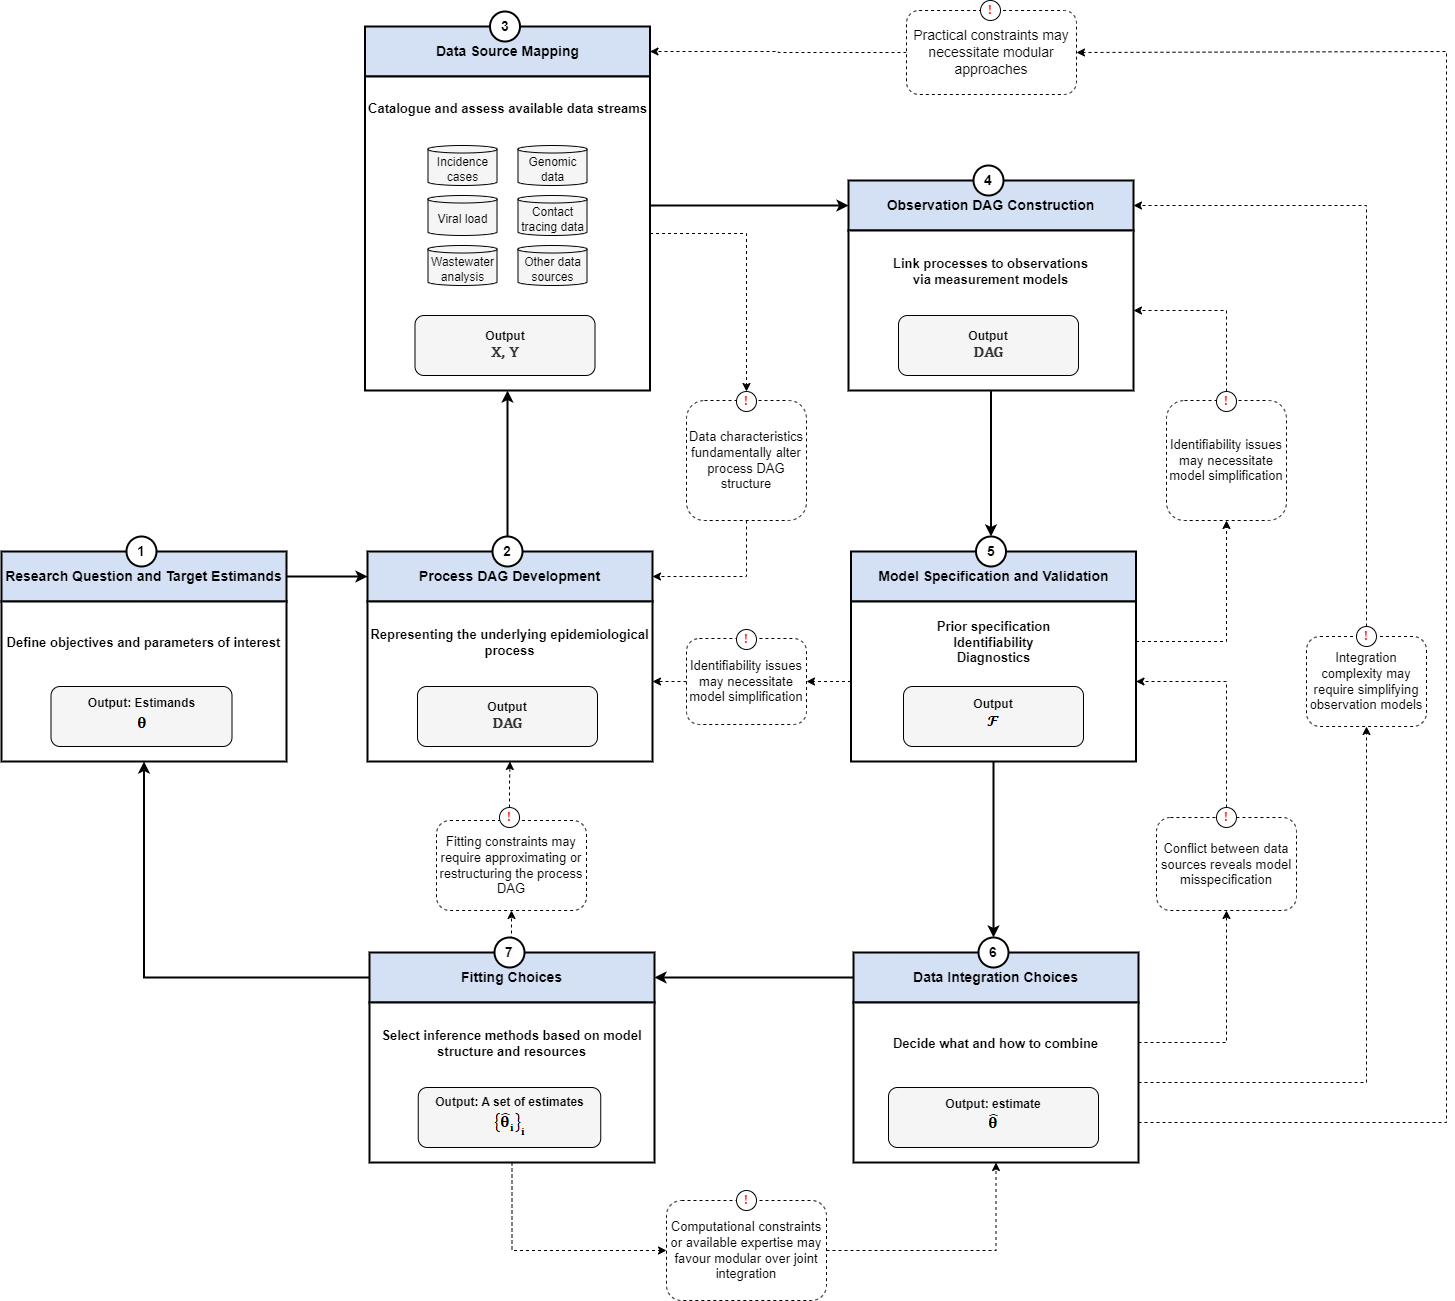
\includegraphics[width=\textwidth]{figures/visualization of core steps.drawio.png}
    \caption{Recommended workflow for integrating multiple data sources in infectious disease modelling. Begin by defining research questions and target estimands, proceed through iterative development of process and observation DAGs, and follow critical decisions about data integration and inference methods. Note the feedback loops where downstream choices constrain or inform upstream model development.}
    \label{fig:workflow}
\end{figure}

Our workflow extends established Bayesian workflow principles—with their emphasis on iterative model building, prior predictive checks, computational diagnostics, and posterior predictive assessment—to the specific challenges of multi-source infectious disease modelling.
A key distinguishing feature is the explicit separation of epidemiological process DAGs from observation DAGs, recognising that whilst these components interact through feedback mechanisms, they draw from different domains: epidemiological processes are informed by infectious disease theory whilst observation models are motivated by data source characteristics and collection mechanisms.
Start with a clear research question—such as estimating transmission intensity—and use systematic model development through directed acyclic graphs (DAGs) with iterative refinement.
We advocate this approach because it makes modelling choices transparent, assumptions explicit, and provides principled tools for assessing model adequacy regardless of whether final inference is Bayesian or frequentist.

We recommend beginning with \textbf{decision making}: clearly define your research question and target estimands (e.g., time-varying reproduction number, overdispersion parameters).
Next, develop a \textbf{process DAG} representing the underlying epidemiological process, iterating on this representation as understanding develops.
Map available \textbf{data sources} to your process model, such as incidence time series, genomic data, contact tracing, viral load measurements, and serological surveys.
For each data source, develop an \textbf{observation DAG} linking the underlying process to observed data through measurement models and reporting mechanisms.
Different data sources may also impact your \textbf{process DAG} assumptions, such as if you can collapse your representation of the process from individual-level to population-level.

Once you have developed your process and observation DAGs, proceed to \textbf{model specification and validation}, including prior specification, parameter identifiability assessment, and diagnostic approaches.
You then face the key decisions: \textbf{"What to combine?"} and \textbf{"How to combine?"}
If combining multiple sources is not beneficial or feasible, you can proceed to single-source modelling and combination of estimates.
If integration is warranted, select among data integration methods including full joint modelling, modular techniques, Markov melding, or approximate weighting approaches.
Finally, fit your model and evaluate its performance through posterior predictive validation and sensitivity analysis.

The workflow can be summarised as follows:

\textbf{Core Workflow Components:}
\begin{enumerate}
    \item \textbf{Research Question and Target Estimands} - Define your objectives and parameters of interest
    \item \textbf{Process DAG Development} - Represent the underlying epidemiological process
    \item \textbf{Data Source Mapping} - Catalogue and assess available data streams
    \item \textbf{Observation DAG Construction} - Link processes to observations via measurement models
    \item \textbf{Model Specification and Validation} - Prior specification, identifiability, diagnostics
    \item \textbf{Data Integration Choices} - Decide what and how to combine
    \item \textbf{Fitting Choices} - Select inference methods based on model structure and resources
\end{enumerate}

\textbf{Key Feedback Loops:}
\begin{itemize}
    \item Components 3→2: Data characteristics (e.g., individual-level vs population-level) fundamentally alter process DAG structure
    \item Components 5→2,4: Identifiability issues may necessitate model simplification
    \item Components 6→3: Practical constraints (e.g., different teams using incompatible programming languages) may necessitate modular approaches
    \item Components 6→4: Integration complexity may require simplifying observation models
    \item Components 6→5: Conflict between data sources reveals model misspecification
    \item Components 7→2: Fitting constraints (e.g., NUTS inability to handle discrete latents) may require approximating or restructuring the process DAG
    \item Components 7→6: Computational constraints or available expertise may favour modular over joint integration
\end{itemize}

These feedback loops mean that model development is rarely a single forward pass through the workflow. For example, if you initially design a joint model but find it computationally intractable with available methods, you might iterate back to choose a modular integration approach, which in turn might influence how you structure your observation DAGs.
Similarly, if MCMC convergence fails due to discrete latent parameters, you might need to marginalise them out or adopt a different process representation.

In the following sections, we will discuss each of these steps in more detail.

\subsection{Research Question and Target Estimands}
% TODO: Defining clear research objectives
% TODO: Specifying target parameters and estimands
% TODO: Connecting questions to policy needs
% TODO: Setting scope and boundaries

\subsection{Process DAG Development}
% TODO: Representing epidemiological processes
% TODO: Causal relationships and assumptions
% TODO: Iterative refinement based on understanding
% TODO: Incorporating biological mechanisms

\subsection{Data Source Mapping}
% TODO: Cataloguing available data streams
% TODO: Assessing data characteristics and biases
% TODO: Linking data to process components
% TODO: Evaluating complementarity and redundancy

\subsection{Iterate on the Process DAG}

%TODO: based on available data sources and the original process DAG may need to iterate
%TODO: An example is the need for individual level modelling for certain data sources which might impact the construction of the process DAG.

\subsection{Observation DAG Construction}
% TODO: Measurement models and reporting processes
% TODO: Delays and missing data mechanisms
% TODO: Linking latent processes to observations
% TODO: Accounting for data collection protocols

\subsection{Model Specification and Validation}\label{sec:spec-validate}
% TODO: Bayesian workflow principles
% TODO: Prior specification and prior predictive checks
% TODO: Parameter identifiability assessment
% TODO: Model criticism and diagnostic approaches
% TODO: Posterior predictive validation
% TODO: Cross-validation strategies
% TODO: Sensitivity analysis frameworks

\subsection{Data Integration Choices}
% Lead: Anne Presanis

%Consideration: How do we clearly split here between combined and individual approaches? What does that structure look like? How do we connect this question to fitting choices which in practice are important?
%Consideration: What parts of this (sub models etc etc are part of specification and validation. How does that interaction work?
%Consideration: There might be an ideal DAG structure but in practice need to approximate for fitting. I.E want to use NUTs so can't have latent discrete parameters etc...

\subsubsection{Decision Framework}
% When to integrate vs when to keep separate
% Assessing complementarity and redundancy
% Computational vs inferential trade-offs

\subsubsection{Integration Methods}
% Full joint modelling
% Modular approaches and staged fitting
% Markov melding
% Ensemble and weighting methods
% Cut distribution and generalised evidence synthesis

\subsubsection{Practical Constraints}
% Different teams with different expertise/languages
% Software compatibility issues
% Computational resource limitations
% Time constraints in outbreak settings

\subsubsection{Conflict Detection and Resolution}
% Prior-data conflict
% Data-data conflict
% Model criticism in multi-source settings
% Sensitivity analysis approaches

Attempt at tree of choices:
\begin{tree}
    \item Are you combining alternative/competing models from different groups?
    \begin{tree}
        \item Yes
        \begin{tree}
            \item How are the results from each available?
            \begin{tree}
                \item As point estimate and confidence/credible interval
                \begin{tree}
                    \item Do you trust the alternatives equally?
                    \begin{tree}
                        \item Yes $\Rightarrow$ standard meta-analysis
                        \item No
                        \begin{tree}
                            \item $\Rightarrow$ weighted meta-analysis, weighted by precision
                            \item $\Rightarrow$ or weighted by other criteria, e.g. prediction accuracy (ensembling)
                        \end{tree}
                    \end{tree}
                \end{tree}
                \item As posterior samples or analytic posterior distribution
                \begin{tree}
                    \item Do you trust the alternatives equally?
                    \begin{tree}
                        \item Yes
                        \item No
                    \end{tree}
                \end{tree}
            \end{tree}
        \end{tree}
        \item No
        \begin{tree}
        \item Are your sub-models independent conditional on their common parameters?
        \begin{tree}
            \item Yes
            \begin{tree}
                \item Do you already have posterior samples from all sub-models?
                \begin{tree}
                    \item Yes
                    \begin{tree}
                        \item Are you already convinced that all sub-models give consistent results?
                        \begin{tree}
                            \item Yes $\Rightarrow$ join all sub-models simultaneously using Markov melding
                            \item No $\Rightarrow$ join the models sequentially using Markov melding, to test for conflict between each sub-model
                        \end{tree}
                    \end{tree}
                    \item No $\Rightarrow$ decide order in which to fit/add each sub-model, e.g. start from the one you trust most, and add sequentially using Markov melding, testing for conflict between each sub-model
                \end{tree}
            \end{tree}
            \item No
        \end{tree}
        \end{tree}
    \end{tree}
\end{tree}

\begin{figure}[htbp]
    \centering
    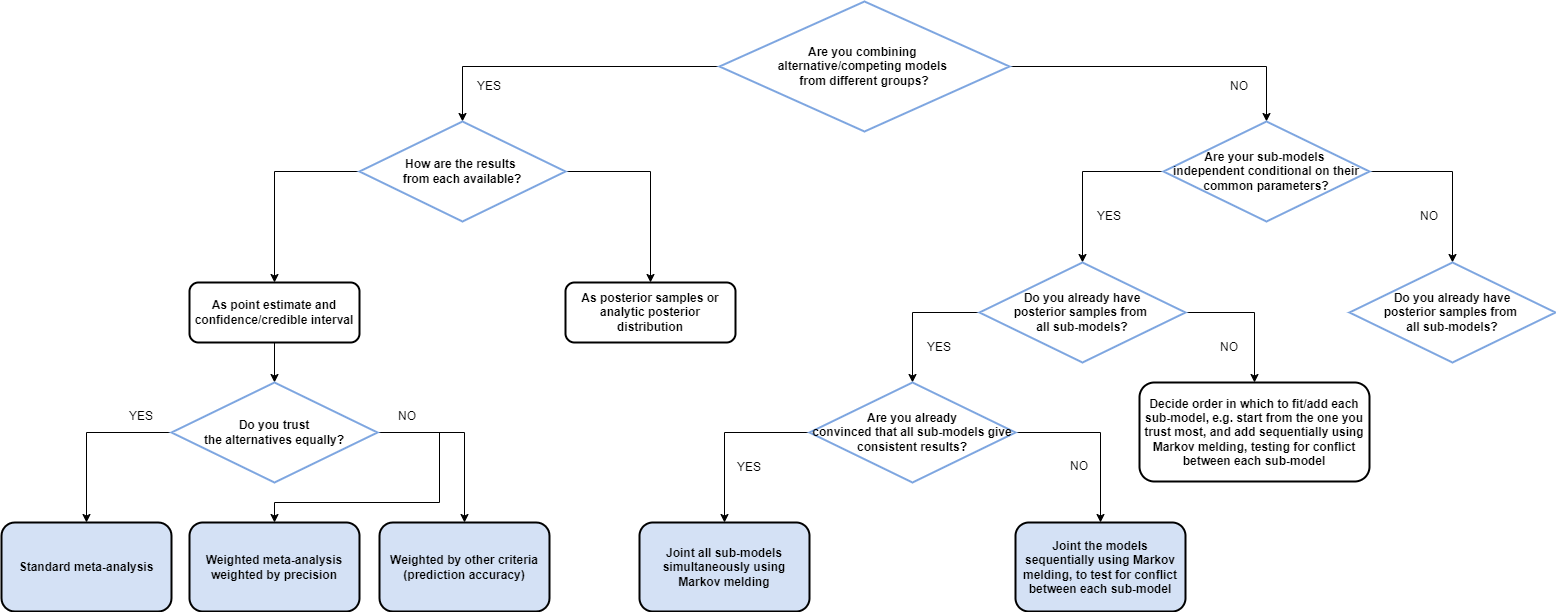
\includegraphics[width=\textwidth]{figures/integration choices decision tree.drawio.png}
    \caption{Decision tree of integration choices for integrating multiple data sources in infectious disease modelling.}
    \label{fig:fitting}
\end{figure}

First stab outline 27/05
\begin{itemize}
    \item Different possible choices for integrating/ensembling inference from multiple data sources
    \begin{itemize}
        \item Full joint model fitted, regardless of whether you have already fitted separate sub-models
        \item Conditionally independent sub-models each fitted separately, then integrated
        \begin{itemize}
            \item Meta-analysis of separate estimates
            \item Weighted averaging / ensembling
            \item Markov melding
        \end{itemize}
    \end{itemize}
    \item Depends on whether you are starting from scratch, from an existing model for one data source to which you want to add others, or whether you have multiple alternative sets of existing inferences from different data sources that you want to combine
    \item General principle that modular model building (De Angelis et al, 2015; Birrell et al, 2018; Goudie et al, 2019; De Angelis \& Presanis, 2019; Gelman et al, 2020; Nicholson et al, 2022, Liu \& Goudie, 2025) is preferable, since:
    \begin{itemize}
        \item Easier to understand lack of fit, model misspecification or convergence issues from simpler sub-models individually
        \item Occam's razor - principle of parsimony, start from simplest model and build complexity up only as far as needed
        \item Adding sub-models in one at a time allows for assessment of consistency/conflict between sub-models sequentially
        \item Computational efficiency - rather than fitting full joint models after fitting the sub-models, use the posterior samples from the sub-models to obtain your full joint model (melding or ?)
    \end{itemize}
    \item Choice of likelihood function (or other objective function) and fitting choices (\ref{sec:fitting}) therefore depends on options above on where you are starting from (existing models/sub-models or from scratch)
    \item And model development is a cycle of model building and model criticism
    \begin{itemize}
        \item extension of model validation in \ref{sec:spec-validate} to multiple data sources setting
        \item detection/measurement of conflict not only between prior and data, but between data and data, or partitions of the DAG (modules) comprising different combinations of prior and data, i.e. posterior-posterior comparisons
        %\item TODO: conflict references from Fuming's literature review
    \end{itemize}
\end{itemize}

% TODO: Add practical examples of each approach
% TODO: Include decision framework for choosing integration method

\subsection{Fitting Choices}\label{sec:fitting}
% Lead: Anne Presanis, with Dhorasso and Xiahui

Inference for infectious disease models typically involves estimating a set of parameters $\theta$ from observed data $Y$, which may include case counts, hospitalizations, deaths, wastewater surveillance or other epidemiological measurements. These data are assumed to arise from a probabilistic model characterized by a likelihood function $p(Y | \theta)$ that links the parameters to the observations through both an underlying disease transmission process and a noisy observation mechanism.  The inferential task depends on whether the likelihood $ p(Y | \theta)$ is tractable (computable analytically or efficiently numerically), intractable (requiring approximation), or unavailable (necessitating likelihood-free, simulation-based methods). This section briefly reviews common computational approaches, emphasizing practical considerations and current best practices. 

\begin{figure}[htbp]
    \centering
    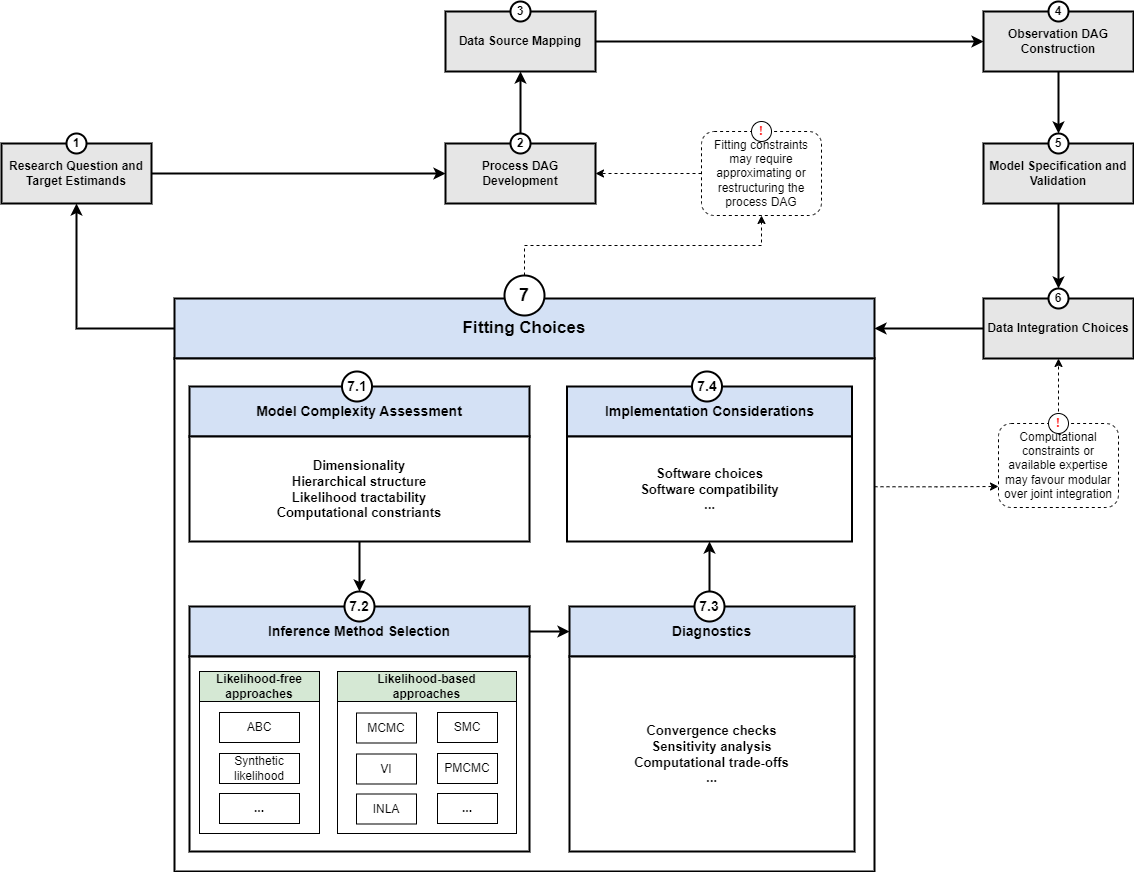
\includegraphics[width=\textwidth]{figures/Subpanel_fitting choices_v2.drawio.png}
    \caption{Fitting choices workflow for integrating multiple data sources in infectious disease modelling.}
    \label{fig:fitting}
\end{figure}

% \subsubsection{Tools for Tractable Likelihood Functions}
% % TODO: MCMC and its variants for joint models
% % TODO: Sequential Monte Carlo (SMC) approaches

% \subsubsection{Tools for Partially Tractable Likelihood Functions}
% % TODO: Particle MCMC (pMCMC) for state-space formulations
% % TODO: Variational inference (VI) and INLA for specific model classes

% \subsubsection{Tools for Intractable Likelihood Functions}
% % TODO: Approximate Bayesian Computation (ABC-MCMC, ABC-SMC)
% % TODO: ABC with history matching
% % TODO: Bayesian Synthetic Likelihood (BSL)
% % TODO: Simulation-based inference approaches



\subsubsection{Likelihood-based methods}
Likelihood-based inference broadly includes both frequentist and Bayesian frameworks. Although classical frequentist methods like maximum likelihood estimation \citep{myung2003tutorial, baltazar2024maximum} and profile likelihood \citep{tonsing2018profile, plank2024structured} provide well-established tools for inferring parameters, we emphasize the Bayesian methods because of their capacity for dealing with uncertainty and flexibility in accommodating various sources of information.

Bayesian inference provides a framework to update prior beliefs $ p(\theta)$ on a parameter upon observing data to obtain a posterior distribution, $p(\theta | Y) \propto p(Y|\theta) \,p(\theta)$. For simple models with the likelihood belonging to theIn models with complex latent state structures, the likelihood function is often computationally intractable. exponential family, there exist conjugate priors that allow for closed-form derivation of posterior distributions and exact Bayesian updates \citep{gelman1995bayesian, lawson2018bayesian, cori2013new}. However, many infectious disease models typically involve complexities that make exact inference infeasible.


When the likelihood can be evaluated (up to a constant) but closed-form posteriors are unavailable, sampling-based Bayesian methods, especially Markov Chain Monte Carlo (MCMC) remain the golden standard approach \citep{gilks1995markov, lekone2006statistical}. Common MCMC methods like Metropolis–Hastings \citep{hastings1970monte} and Gibbs sampling \citep{geman1984stochastic}, require evaluating the posterior up to a constant. For latent variable models, data-augmented MCMC can be used to include auxiliary states and infer parameters as well as the hidden variables \citep{o1999bayesian}. Improved techniques such as Hamiltonian Monte Carlo (HMC) for differentiable likelihoods \citep{duane1987hybrid} and their adaptive variant No-U-Turn Sampler (NUTS) \citep{hoffman2014no, andrade2020evaluation}, achieve more efficient sampling by using gradient information and automatic hyperparameter tuning.  Other approaches such as Variational Inference (VI) provide a scalable, faster alternative to MCMC by maximizing a tractable approximation of the posterior distribution at the cost of some bias \citep{blei2017variational, chatzilena2019contemporary}.


In state-space models with high-dimensional latent state structures, the likelihood function is often computationally intractable due to the need to marginalise over the latent states. Sequential Monte Carlo (SMC) or particle filter overcomes this by approximating the posterior distribution of latent states as a set of weighted particles and producing an unbiased estimate of likelihood \citep{doucet2001introduction, arulampalam2002tutorial}. This approximation can be integrated into an MCMC framework process to form the particle MCMC (PMCMC) \citep{andrieu2010particle, endo2019introduction} to facilitate joint parameter and latent state inference. Sequential Monte Carlo Squared (SMC$^2$) \citep{chopin2013smc2} takes it one step further in performing fully sequential Bayesian updating as observations are accumulated.

\subsubsection{Likelihood-Free Methods}

While likelihood-based methods are powerful for parameter inference, they rely on the ability to evaluate the likelihood function, which can be computationally intractale or analytically unavailable for complex infectious disease models. Likelihood-free methods tackle this challenge by simulating from the model rather than directly evaluating likelihood.

Approximate Bayesian Computation is a widely used likelihood-free method that approximates the posterior distribution by accepting parameter values that produce simulated data close to the observed data under a predefined distance metric \citep{rubin1984bayesianly, tavare1997inferring, beaumont2002approximate}. While conceptually simple, the classical ABC rejection sampling suffers from inefficiency in high-dimensional parameter or data spaces. To address this limitation, advanced ABC variants have been developed. 

ABC-MCMC combines ABC with MCMC to explore the parameter space more efficiently. By using a proposal distribution and a Metropolis-Hastings acceptance step alongside a simulation-based criteria, ABC-MCMC enhances efficiency for peaked or correlated posteriors \citep{marjoram2003markov, wegmann2009efficient, kypraios2017tutorial}. However, its performance is sensitive to the choice of tolerance thresholds and proposal distributions.

ABC-SMC iteratively refines the tolerance and proposal distributions across a sequence of generations, adaptively concentrating computational effort on high-probability regions of the parameter space \citep{sisson2007sequential, toni2009approximate, beaumont2009adaptive, drovandi2011likelihood}. This approach performs well in handling multi-modal posteriors better than ABC-MCMC.

When exact likelihoods are unavailable but the model can be simulated repeatedly, synthetic likelihood methods provide an alternative by approximating the likelihood via assuming Gaussian distributions for summary statistics \citep{wood2010statistical, price2018bayesian}. 

\subsubsection{Selecting the Right Tool}
% TODO: Trade-offs between computational complexity, accuracy, bias
% TODO: Interpretability and implementation ease considerations
% TODO: Decision-making frameworks for method selection

Choosing the most appropriate inference method requires balancing the trade-offs between computational constraints, statistical rigor, data availability, interpretability and model complexity  \citep{funk2020choices}. Rather than adopting a one-size-fits-all approach, the choice should be tailored to the modeling context and inferential goals. 

MCMC-based methods naturally incorporate prior knowledge and generate samples that, under suitable conditions, approximate the exact posterior distribution. This is critical for interpreting epidemiological parameters and accurately propagating uncertainty. However, Bayesian inference with such methods can be computationally intensive in highly complex or high-dimensional mechanistic models. When computational resources are limited, for instance for the monitoring of an outbreak in real-time or when analyzing very large data sets, approximate inference methods like VI or ABC-SMC might offer scalable alternatives \citep{chatzilena2019contemporary, engebretsen2023real}.

Aside from computational efficiency, statistical accuracy is also a concern. Regardless of method, the accuracy of parameter estimates is largely a function of algorithmic setup such as prior distributions, tuning parameters, tolerance threshold, and the number of particles or iterations used. Methods based on full likelihoods generally offer higher accuracy subject to likelihood tractability and proper specification, whereas likelihood-free approaches may often prioritise flexibility and scalability over precision. 

Interpretability and ease of implementation is also to be taken into account while making the choice. Certain methods,  can be easier to implement and debug within default probabilistic programming environments, but others, may require further tuning and computational expertise. Ultimately, selecting the right tool is guided by a systematic decision process considering the purpose for the modeling, the urgency or latency constraints, the system complexity, and available computational capabilities. Model checking, sensitivity analysis, and validation continue to be required regardless of the approach taken. These steps are aimed at ensuring that the inferences drawn are not only statistically valid but are also scientifically plausible and decision-useful.


\subsubsection{Practical Implementation}
% Lead: Sam Abbott
% TODO: Software implementations and availability
% TODO: Diagnostic tools and convergence assessment
% TODO: Computational resource requirements
% TODO: Reference to inference subpanel workflow figure

\section{Case Studies}
% Lead: Anne Cori

\subsection{Overview}

We demonstrate our iterative workflow through four progressive case studies, each building complexity whilst showing different integration choices and methodological considerations.
All case studies share common estimands -- the time-varying reproduction number ($R_t$) and overdispersion parameter ($k$) -- using SARS-CoV-2 outbreak data to leverage expert survey evidence on data source characteristics.
Each case study follows our complete workflow framework, demonstrating how different data sources enable analyses to answer questions that would otherwise require strong assumptions.

The progression illustrates key principles: data on deaths eliminate reporting fraction assumptions that plague case-only analyses; wastewater eliminates testing bias inherent in symptomatic surveillance; individual-level data enables direct overdispersion estimation without distributional assumptions.
Implementation choices reflect practical considerations including available expertise, computational resources, time availability, and model complexity trade-offs, whilst generally favouring efficient methods like NUTS where applicable.

TODO: need to add something on data source mapping which all the case studies will draw from: what data are available that may inform Rt and superspreading estimates? (Can draw from the survey and Anne C's slides at CIRM). What are their pluses and minuses (if we cannot do the full mapping from survey we can still discuss - otherwise refer to that section).

\subsection{Case Study 0: Single-Source Baseline (Cases Only)}

This case study showcases the workflow and explores some of the assumptions and modelling and fitting choices underlying estimation of $R_t$ from a single time series of case incidence using a simple branching process model.

%\textbf{Research Question:} What is Rt during this outbreak period using case incidence alone?

\textbf{Question:} What is $R_t$ during this outbreak period?

%\textbf{Workflow Demonstration:}
%\begin{enumerate}
%    \item \textbf{Process DAG:} Simple renewal equation linking Rt to case incidence through generation time distribution, incorporating overdispersion via negative binomial model
%    \item \textbf{Data Source Mapping:} Case incidence time series selected based on expert survey ratings showing high timeliness but moderate precision due to testing policy effects
%    \item \textbf{Observation DAG:} Reporting delays, underascertainment fraction, weekend reporting effects
%    \item \textbf{Integration Choice:} Single source (no integration required)
%    \item \textbf{Implementation:} NUTS sampling of renewal equation with negative binomial observation model, chosen for computational efficiency and robust performance
%\end{enumerate}

%\textbf{Key Limitation:} Establishes baseline uncertainty but requires strong assumptions about generation time distribution and reporting fraction, highlighting assumption-dependent limitations that motivate multi-source approaches.

\textbf{Process model}:
 
We consider three variants of the renewal process model for the number of new infections $I_t$ on day $t$, which is influenced by the instantaneous reproduction number $R_t$ on day $t$, and the generation time (GT) distribution, which we assume to be fixed. The three model variants are:
\begin{itemize}
    \item[P1.] No variance in daily infection incidence (deterministic)
    \begin{equation}
        I_t = R_t \sum_{s=1}^\infty I_{t-s}w_s 
    \end{equation}
    \item[P2.] Poisson-distributed daily infection incidence.
        \begin{equation}
        I_t \sim \mathrm{Poiss}\left( R_t \sum_{s=1}^\infty I_{t-s}w_s  \right)
    \end{equation}
    \item[P3.] Negative binomially distributed daily infection incidence. 
            \begin{equation}
        I_t \sim \mathrm{NegBin}\left( R_t \sum_{s=1}^\infty I_{t-s}w_s, k  \right)
    \end{equation}
\end{itemize}
where $w_s$ is the probability mass function for the GT distribution and $k$ is the dispersion parameter. 
The process DAGs for these three models are shown in Figure \ref{fig:CS0_DAGs}.

 
\textbf{Data source mapping}: Case incidence {\color{red} I think we might have agreed to move this to a separate section earlier on rather than covering it within each case study?}
\begin{itemize}
    \item pros: often available easily (cheap, scales well) with very frequent (often daily) updating and high timeliness
    \item cons: imperfect proxy for infection incidence which highly depends on testing policies
\end{itemize}

\textbf{Observation model}:

The observation model relates the observed data (here daily case incidence) with underlying latent variables (here daily infection incidence). 
This requires assumption to be made about underreporting (what fraction of infections are detected cases), reporting delays (time between infection and a case being detected and reported), and random noise (typically used to capture other things not explicitly specified in the model).

Alternative versions of the observation model can be considered, which either ignore or include each of these three aspects. This leads to $2^3=8$ possible observation models, each of which has an associated DAG (but again some DAGs may be the same).
We refer to these models as $O_{000}$ (for the simplest observation model not modelling any of the above) to $O_{111}$ (for the most comprehensive accounting for all three observation features).

\textbf{Fitting and integration approach}:

As there is only one data source in this case study, no decisions about what and how to combine multiple sources are needed. The choice of fitting method may depend on considerations such as analytical tractability of the combined process and observation model, computational complexity and speed of computation relative to the time available, and identifiability issues. 
 
% \begin{itemize}
%     \item Fitting choice discussion points to add:
%     \item Analytically tractable or not. Depends on the specific choices of PRIOR, P and O, the resulting model has an analytic formulation or not which guides choice here
%     \item Identifiability issues
%     \item Computational complexity / speed of computation
% \end{itemize}

One possibility is to consider model ensembling, where multiple estimates of the target estimand (in this case $R_t$) are produced by different groups or methods and synthesised into a combined estimate. [***Link to SPI-M paper from Oxford]. In this context, it may be desirable to align the assumptions made by different models, for example about the GT distribution or the temporal smoothness in $R_t$, to ensure that estimates from the different models are  comparable [***Johannes’ paper].

\textbf{Implementation}:

Implementation requires selection of one process model, one observation model and one fitting and integration method (which will depend on the choice of process and observation model as described above). For this case study, combinations of the 3 process models and 8 observation models give 24 possible models, on top of which alternative fitting methods can be chosen for each. Here, we give a few examples from the literature:
\begin{itemize}
    \item EpiEstim. This method assumes Poisson distributed infections, no underreporting, no delays in reporting, and no observation noise \citep{cori2013new}. In our categorisation, this corresponds to process model P2 and observation model $O_{000}$. The model is fitted by calculating an analytic posterior distribution for $R_t$ from a conjugate prior, which is fast and computationally efficient. 
    \item EpiNow2 [***may need to specify a version]. This method assumes deterministic infection incidence with no underreporting, but with delays and random observation noise. In our categorisation, this corresponds $P_1-O_{011}$. This is fitted using XXX.
    \item Epidemia or EpiMap for NB process – TODO: check what they do!
\end{itemize}

Other possible choices of fitting methods that could be considered / why not (refer to relevant section in the overall framework description)
 
TODO: add a Figure. This will be A visual of jigsaw puzzle presenting a library of P (process models), O (observation models) and F (fitting methods). In multi-data ones we will need to add an I (integration method) too.
Example choices of EpiEstim and EpiNow2 for example (as above). Prototype figure below

\begin{figure}
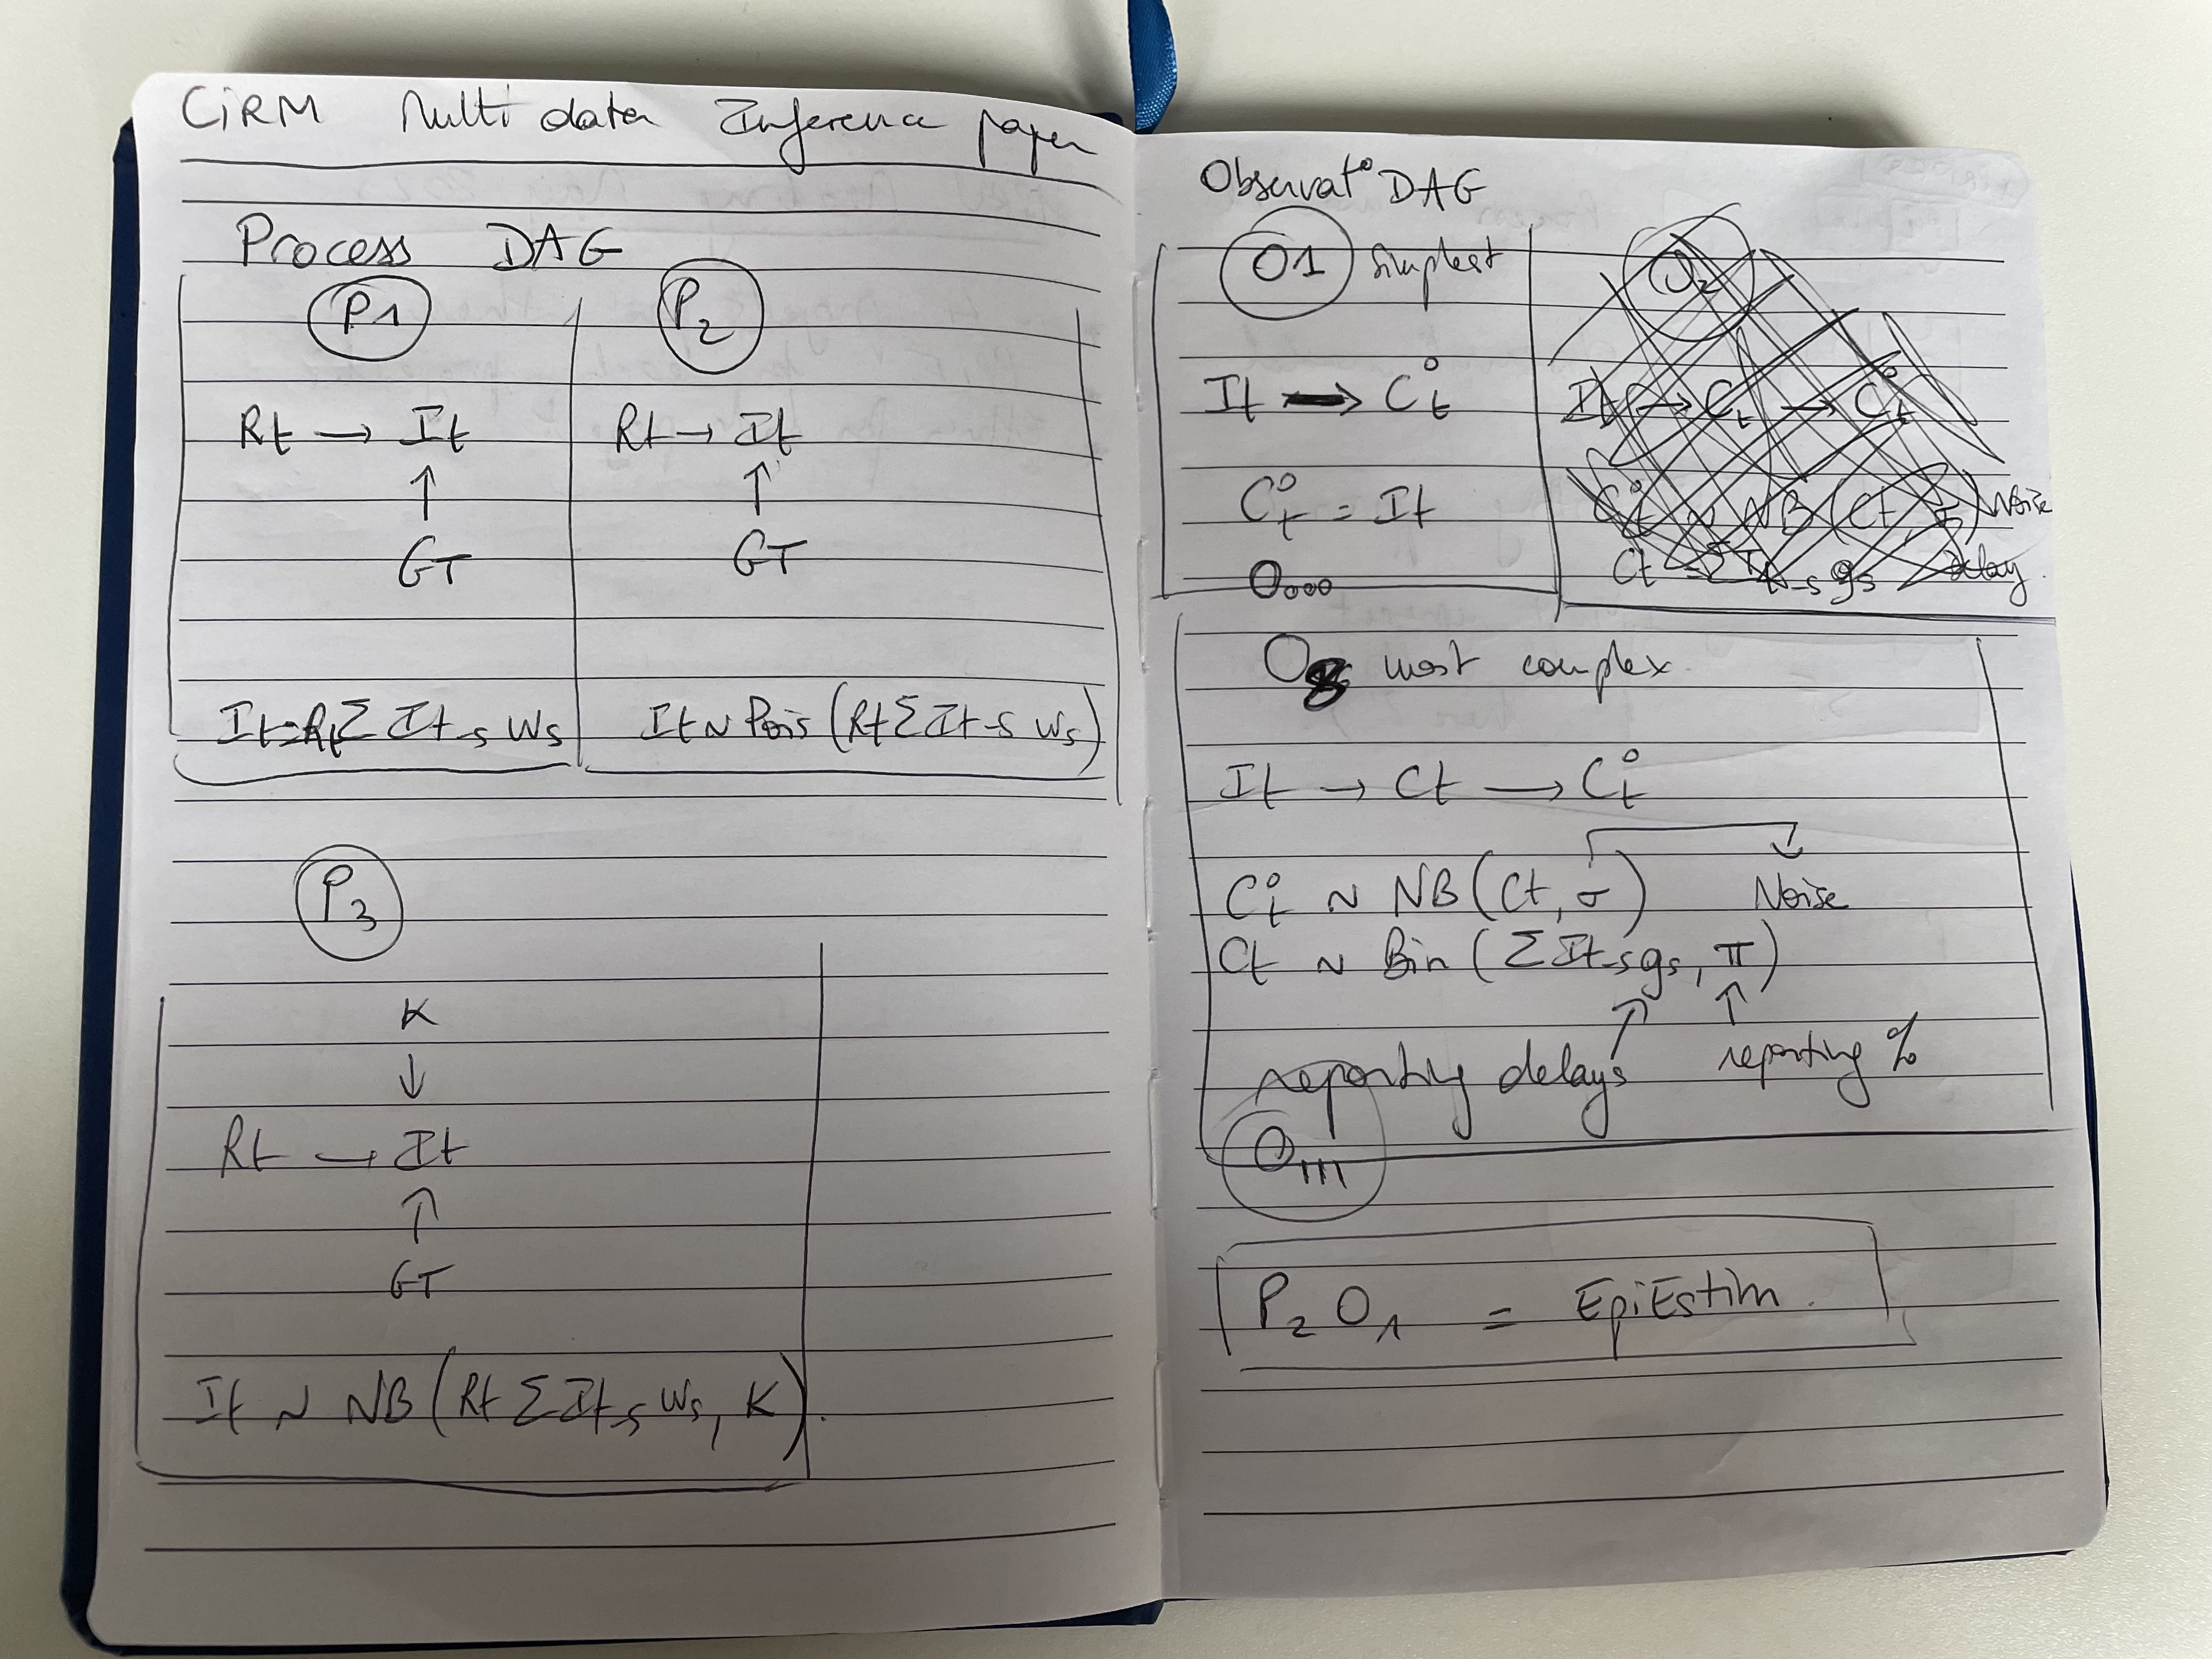
\includegraphics[width=0.75\textwidth]{figures/cs0_diagram1.jpg}
\label{fig:CS0_DAGs}
\end{figure}

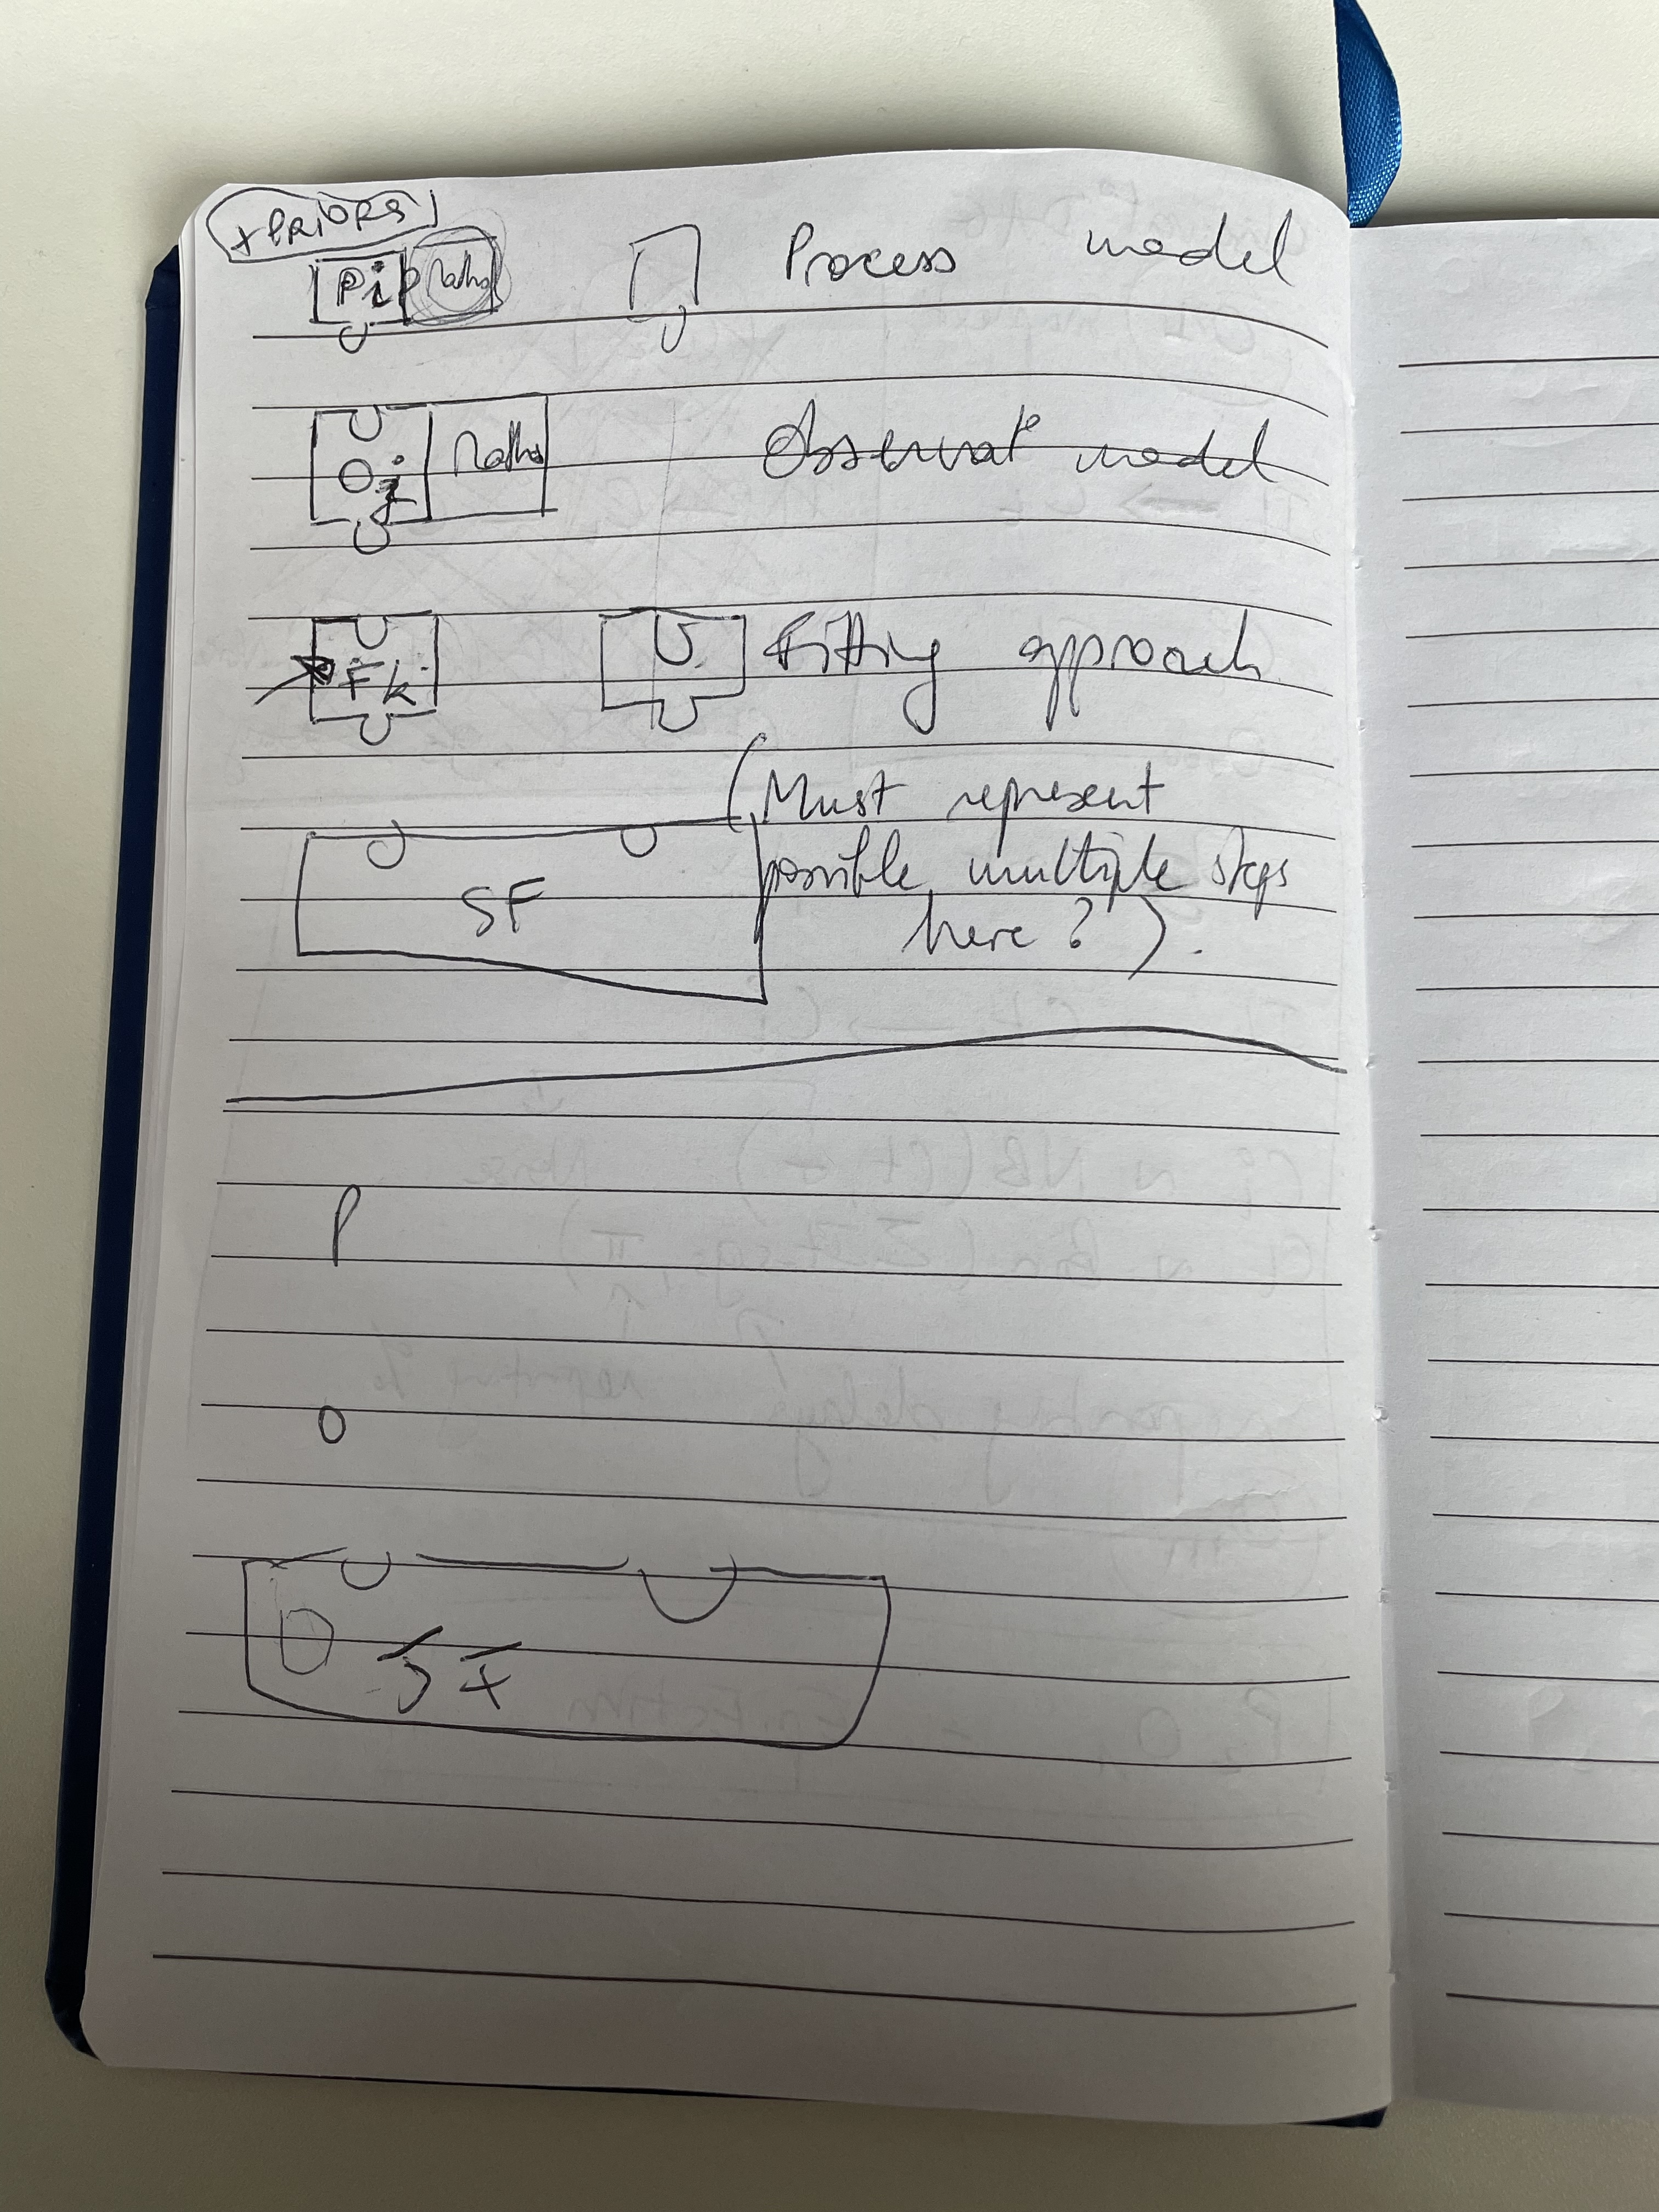
\includegraphics[width=0.75\textwidth]{figures/cs0_diagram2.jpg}

\begin{figure}[htbp]
    \centering
    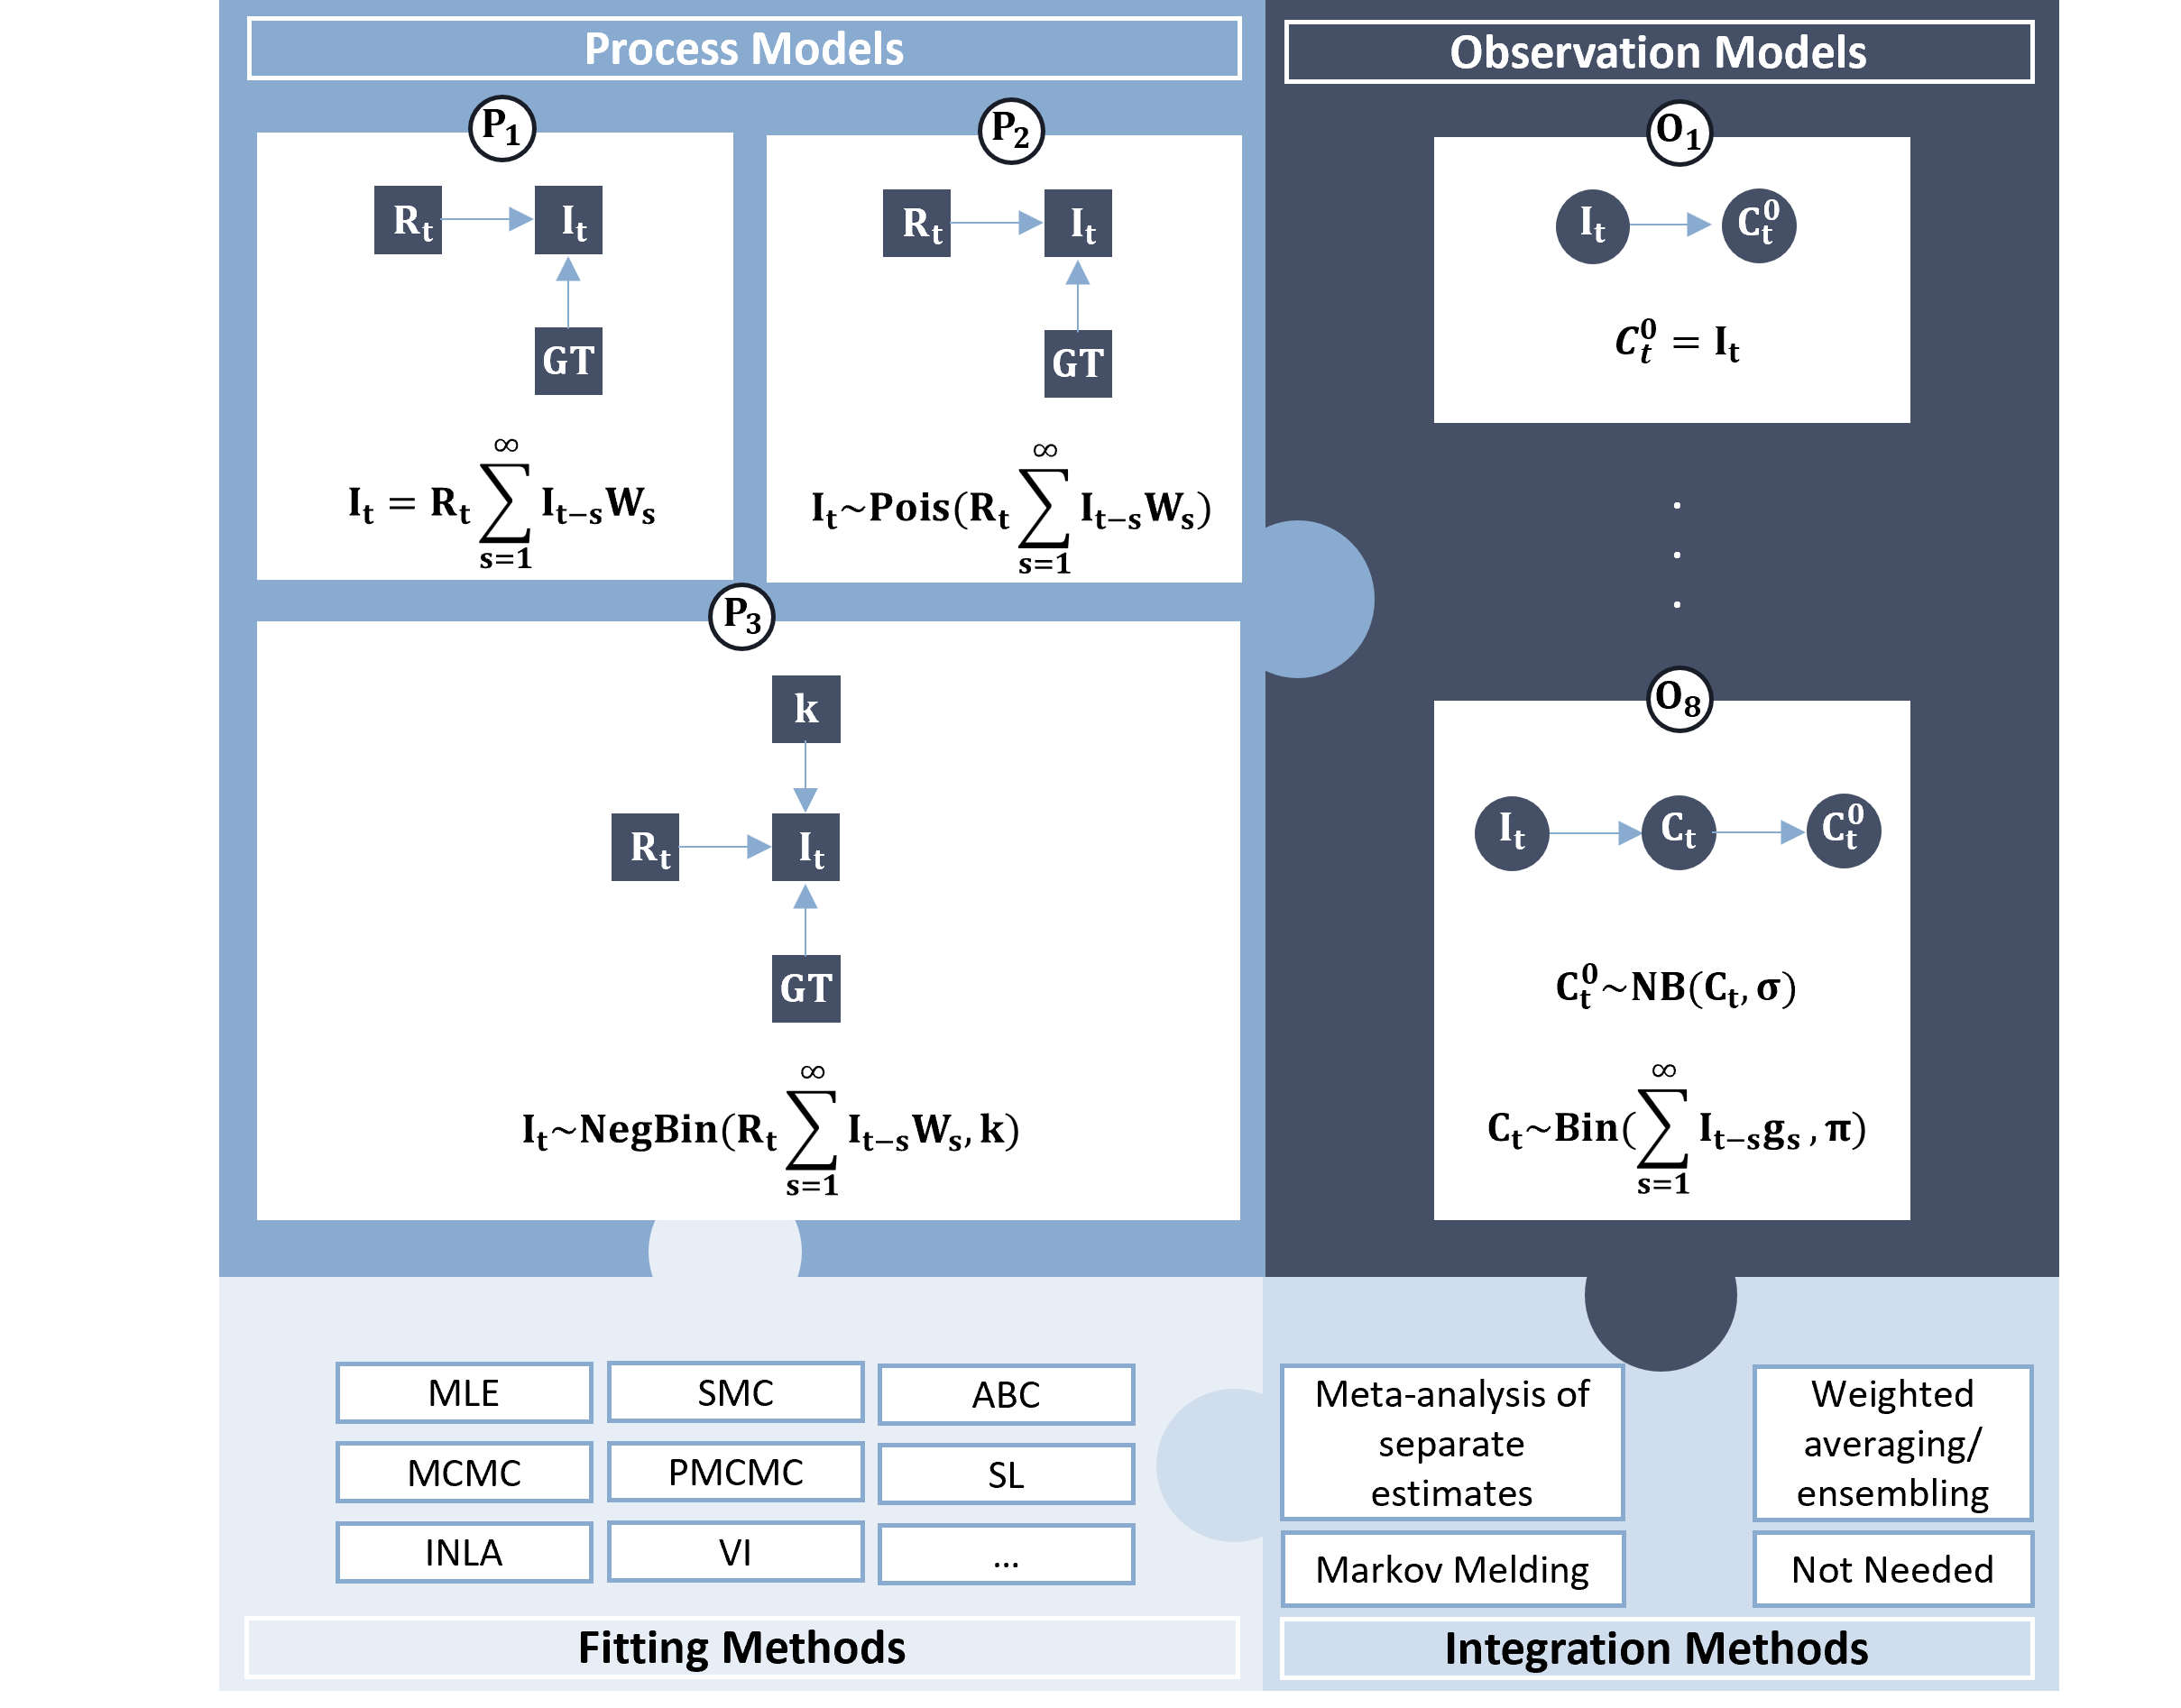
\includegraphics[width=\textwidth]{figures/Case study puzzle.png}
    \caption{A visual of jigsaw puzzle presenting a library of process models, observation models, integration methods, and fitting methods.}
    \label{fig:case_study_visual}
\end{figure}

\textbf{Question to Anne P} – can we write the model (e.g. assuming Poisson likelihood) as part of the DAG or is that something separate? If separate then we should make it clear throughout that the DAG isn’t the full model spec.

Different approaches have different strengths and limitations. For example, the key strength of EpiEstim is computational speed, whereas its key weaknesses are ignoring underreporting and reporting delays. The first of these may be less important in contexts where the reporting fraction can reasonably be assumed to be steady over the time period of interest. Furthermore, any change in reporting fraction will not be identifiable from a case time series alone, so it would not be sensible to attempt to estimate this in this example. EpiNow2 overcomes some of these weaknesses, at the cost of increased computational complexity. The more appropriate option may depend on the balance between need for timely estimates (e.g. for modelling an outbreak in real-time) and the realism of the associated assumptions. 

A common weakness of all the models outlined above is that they assume the GT distribution is constant and perfectly known. Some approaches (e.g. some versions of EpiEstim) extend the approach to relax this assumption (see also Case Study 4).
 
\textbf{Next steps}:
\begin{itemize}
    \item feedback from others on case study 0
    \item Anne C to draft similar case study 1 (cases + deaths)
    \item Someone with skills to make nice picture of my horrific handwritten plots
\end{itemize}

\subsection{Case Study 1: Two-Source Integration (Cases and Deaths)}

\textbf{Research Question:} How does adding death data improve $R_t$ estimation and reduce assumption dependence?

\textbf{Workflow Demonstration:}
\begin{enumerate}
    \item \textbf{Process DAG Iteration:} The number of deaths $D_t$ on day $t$ depends on the time series of infections up to day $t$, the infection-fatality ratio $p_d$, and the distribution $v_s$ of time from infection to death. This can be represented in the process DAG (Figure X) and by the following convolution equation:
    \begin{equation} \label{eq:Dt}
        D_t \sim \mathrm{Poiss}\left(p_d \sum_{s=1}^\infty I_{t-s}v_s \right)
    \end{equation}
    Other process models for deaths are possible, for example using a multinomial model for the number of deaths occurring on day $s+k$ due to infections on day $s$ ($k=1,2,\ldots$). However, the Poisson model is a good approximation provided $p_d\ll 1$.
    Eq. \eqref{eq:Dt} assumes that the probability $p_d$ of an infection resulting in death and the distribution of time from infection to death are fixed and known.
    
    Eq. \eqref{eq:Dt} describe the probability of deaths conditional on infections $P(D | I)$ and would typically be used in combination with one of eq. P1-P3 \textcolor{red}{[NEED TO HARMONISE NOTATIONS FOR EQUATIONS]} that describe the dynamics of infections $P(I)$, to produce a joint model $P(D, I)$. 
    \item \textbf{Data Source Mapping:} Expert survey shows deaths have higher reporting delays but lower noise (e.g. due to "day-of-the-week" reporting effects) and less policy dependence than cases (e.g. due to changing testing patterns)
    \item \textbf{Observation DAG:} Similar to the different choices of observation model for cases described in case study 0 (and still relevant to this case study), the observation model for deaths could include underreporting, reporting delays, and random noise. In jurisdictions with comprehensive death records, it may be reasonable to assume all deaths are reported and there is no additional noise, but it may still be important to account for delays, for example delay from date of occurrence to date of registration. This would corresponds to observation model $O_{010}$.
    \item \textbf{Integration Choice Comparison:} 
       Two different approaches are possible for integration: (1) a joint model including both cases and deaths with a shared latent state $R_t$; (2) separate models for cases and deaths, resulting in two estimates for $R_t$ to be combined via a weighted ensemble. 
       
       As outlined above, we recommend fitting separate models to the two time series initially, to understand their behaviour and reveal whether they lead to consistent or conflicting estimates of $R_t$. Where inconsistent results emerge, these could lead to refinement of the model (i.e. going back to step 1); for example should $R_t$ estimates show similar trends but shifted in time, assumptions about delays may be revisited. Once this has been done, it may be desirable to combine the results into a single estimate by ensembling, or to fit a joint model that produces a single estimate from both data sources.  
       
    \item \textbf{Implementation:} For separate models, a good choice would be NUTS for estimation, followed by Markov melding to ensemble the results from the two models. For a joint model, a numerical method such as particle MCMC would likely be needed due to the state-space formulation complexity.

    \textcolor{red}{I think we should add some examples from the literature here. Just adding some notes for now:} 1) EpiNow2 seems to allow fitting jointly to cases and deaths: \url{https://wellcomeopenresearch.org/articles/5-112} - they use P1 for infections, but not very clear about cases and deaths - would need Sam's help here 2) this has several models based just on deaths - the last one uses cases and deaths but I don't think has a mechanisms for cases changing over time \url{https://journals.plos.org/plosone/article?id=10.1371/journal.pone.0286199} 3) I think Epidemic uses only deaths actually \url{https://static-content.springer.com/esm/art%3A10.1038%2Fs41586-020-2405-7/MediaObjects/41586_2020_2405_MOESM1_ESM.pdf}

    \end{enumerate}

\textbf{Key Insight:} In case study 0 using data on cases alone, the case ascertainment rate (i.e. the proportion of infections that are reported as cases) was non-identifiable and had to be assumed. Including data on deaths, if the infection-fatality ratio is known, means that the case ascertainment rate could be included as a target for estimation. However, this requires assumptions about the distribution of time from infection to death, demonstrating how additional data sources can shift rather than eliminate the need for modelling assumptions.




\subsection{Case Study 2: Three-Source Integration (Cases, Deaths and Wastewater)}

\textbf{Research Question:} How do we handle conflicting signals between data sources and incorporate complex observation processes?

\textbf{Workflow Demonstration:}
\begin{enumerate}
    \item \textbf{Process DAG Iteration:} Add viral shedding pathway from infections to wastewater concentration
    \item \textbf{Data Source Mapping:} Wastewater offers population-level signal independent of testing bias, with moderate timeliness but requiring environmental expertise
    \item \textbf{Observation DAG:} Complex shedding model incorporating individual-level variation, catchment population dynamics, environmental degradation
    \item \textbf{Integration Choice:} Modular approach with sequential consistency assessment to detect and resolve data source conflicts. Or joint model with shared Rt parameter. 
    \item \textbf{Implementation:} ABC-SMC for wastewater sub-model due to likelihood intractability, reflecting available environmental modelling expertise; NUTS for case/death models. Or particle MCMC for joint model.
\end{enumerate}

\textbf{Key Insight:} Wastewater enables trend detection independent of testing policy but requires environmental and shedding assumptions, whilst modular approach facilitates conflict detection between data sources.

\subsection{Case Study 3: Individual-Level Data (Cases and Transmission Pairs)}

\textbf{Research Question:} How does individual-level data improve overdispersion estimation and change modelling assumptions?

\textbf{Workflow Demonstration:}
\begin{enumerate}
    \item \textbf{Process DAG Transformation:} Shift from population-level renewal equation to individual-level transmission process with explicit contact structure
    \item \textbf{Data Source Mapping:} Contact tracing provides transmission pairs with direct overdispersion information, contingent on tracing system quality
    \item \textbf{Observation DAG:} Observation probability for transmission pairs, contact tracing coverage and delay effects
    \item \textbf{Integration Choice:} Hierarchical model linking individual transmission events to population-level reproduction number
    \item \textbf{Implementation:} NUTS with data augmentation for unobserved transmissions, chosen for efficient handling of discrete latent variables
\end{enumerate}

\textbf{Key Insight:} Individual-level data enables direct overdispersion estimation without distributional assumptions but requires contact tracing completeness assumptions, demonstrating how data granularity can fundamentally change model structure and inference requirements.

\section{Discussion}

\subsection{Summary}

We have presented a framework for integrating multiple data sources in infectious disease modelling that emphasises practical implementation through a structured, iterative workflow.
Our approach combines systematic model development using directed acyclic graphs with modular integration strategies that prioritise parsimony, interpretability, and explicit assessment of data source conflict.
The framework progresses from clear research question definition through process and observation DAG development to informed choices about integration methods, supported by expert survey evidence on data source characteristics and worked case studies demonstrating progressive complexity.
Key contributions include the structured workflow that makes modelling assumptions transparent, the expert consensus on data source trade-offs that guides selection decisions, and practical guidance that bridges the gap between methodological advances and real-world implementation challenges.
Our modular approach incentives building complexity incrementally, allowing practitioners to assess the value of additional data sources systematically whilst maintaining computational tractability and model interpretability.

\subsection{Strengths and Limitations}
% TODO: Strengths: Modular framework, practical focus, worked examples
% TODO: Strengths: Integration of diverse methodological approaches
% TODO: Strengths: Expert survey and empirical evidence base
% TODO: Limitations: Model selection and validation challenges
% TODO: Limitations: Dependence on data quality and availability
% TODO: Limitations: Computational considerations and scalability

\subsection{Comparison with Existing Literature}
% TODO: Position relative to pipeline vs joint modelling literature
% TODO: Relationship to evidence synthesis and meta-analysis methods
% TODO: Comparison with ensemble forecasting approaches
% TODO: Distinguish from existing reviews and methodological papers
% TODO: Compare with other multi-source integration frameworks

\subsection{Outstanding Challenges and Future Directions}
% TODO: Real-time implementation constraints and solutions
% TODO: Computational scalability for large-scale integration
% TODO: Methodological gaps in current approaches
% TODO: Emerging data sources and integration needs
% TODO: Community standards and best practices
% TODO: Research priorities and next steps

\section{Conclusions}

Integrating multiple data sources offers substantial benefits for infectious disease modelling, but requires careful consideration of trade-offs between information gain, computational complexity, and interpretability.
Our framework provides infectious disease modellers with practical tools for navigating these choices through structured workflows, expert consensus on data characteristics, and demonstrated case studies that progress from single-source baselines to complex multi-stream integration.
The modular approach we advocate offers a pragmatic path forward that balances methodological rigor with practical considerations.
By making modelling assumptions explicit through DAG-based development and providing clear guidance on integration method selection, this framework enables more transparent, reproducible, and effective multi-source modelling.
We recommend that the infectious disease modelling community adopt these structured approaches and work towards establishing community standards for data integration that prioritise both methodological best practices and practical implementation needs.

\section{Acknowledgements}

All <placeholder> workshop participants for useful discussion and feedback. Poppy the dog for making sure to ask the important questions.

\bibliographystyle{plainnat}
\bibliography{references}


\end{document}
